\documentclass[DIN, pagenumber=false, fontsize=11pt, parskip=half]{scrartcl}

\usepackage{ngerman}
\usepackage[utf8]{inputenc}
\usepackage[T1]{fontenc}
\usepackage{textcomp}
\usepackage{amsmath}
\usepackage{amsfonts}
\usepackage{tikz}
\usepackage[hidelinks]{hyperref}
\usepackage{caption}
\usepackage{subcaption}
\newcommand{\ofatdot}{\mathbin{\tikz{\draw[line width=0.25pt] (0,0) circle[radius=0.7ex];\draw[fill] (0,0) circle[radius=0.3ex];}}}


% for matlab code
% bw = blackwhite - optimized for print, otherwise source is colored
\usepackage[framed,numbered,bw]{styles/exercise}

% for other code
%\usepackage{listings}

\setlength{\parindent}{0em}

% set section in CM
\setkomafont{section}{\normalfont\bfseries\Large}

\newcommand{\mytitle}[1]{{\noindent\Large\textbf{#1}}}
\newcommand{\mysection}[1]{\textbf{\section*{#1}}}
\newcommand{\mysubsection}[2]{\romannumeral #1) #2}


%===================================
\begin{document}

\noindent\textbf{Very Deep Learning} \hfill \textbf{Technische Universität Kaiserslautern} \\
WS 2022/23 \hfill Dr. Muhammad Zeshan Afzal \\

\mytitle{Exercise 3 - Recurrent Networks and NLP (Solution)}

\textbf{Deadline: 12.12.2022 \hfill Total Marks: 30}

%===================================
\mysection{3.1. Backpropagation through Time\hfill[4+4=8]}

Consider the following RNN:

\begin{figure}[h]
    \centering
    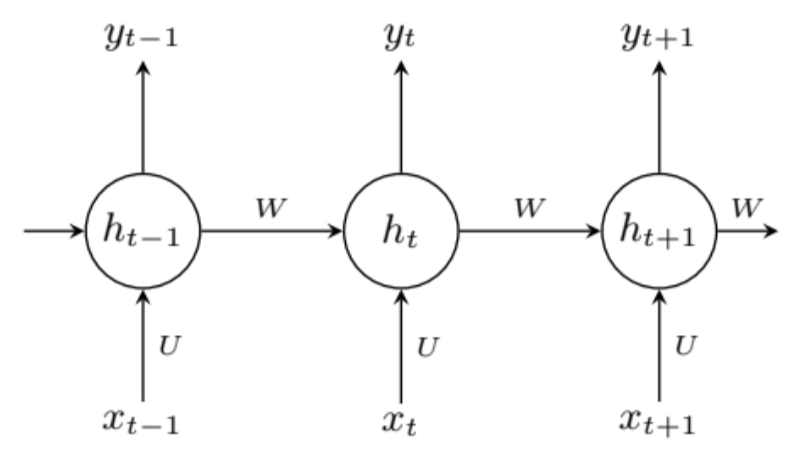
\includegraphics[width=0.5\linewidth]{img/3.1.png}
\end{figure}

Each state $h_t$ is given by:

\begin{equation*}
    h_t = \sigma(W h_{t-1} + Ux_t), \quad \sigma(z) = \frac{1}{1 + e^{-z}}
\end{equation*}

Let $L$ be a loss function defined as the sum over the losses $L_t$ at every time step until time $T: L = \sum^T_{t=0} L_t$, where $L_t$ is a scalar loss depending on $h_t$.

In the following, we want to derive the gradient of this loss function with respect to the parameter $W$.

\newpage
\mysubsection{1}{Given $y = \sigma(W x)$ where $y \in \mathbb{R}^n, x \in \mathbb{R}^d$ and $W \in \mathbb{R}^{n\times d}$. Derive the Jacobian $\frac{\partial y}{\partial x} = diag(\sigma')W \in \mathbb{R}^{n\times d}$.}

\newpage
\mysubsection{2}{Derive the quantity $\frac{\partial L}{\partial W} =
\sum^T_{t=0} \sum^t_{k=1} \frac{\partial L_t}{\partial h_t} \frac{\partial h_t}{\partial h_k} \frac{\partial h_k}{\partial W}$.}

%===================================
\newpage
\mysection{3.2. Vanishing/Exploding Gradients in RNNs\hfill[2+3=5]}

In this exercise, we want to understand why RNNs are especially prone to the Vannishing/Exploding Gradients problem and what role the eigenvalues of the weight matrix play. Consider part 3.1(ii) again.

\mysubsection{1}{Write down $\frac{\partial L}{\partial W}$ as expanded sum for $T = 3$. You should see that if we want to backpropagate through $n$ timesteps, we have to multiply the matrix $diag(\sigma')W$ $n$ times with itself.}

%\mysubsection{2}{Remember that any diagonalizable (square) matrix $M$ can be represented by its eigendecomposition $M = Q\Lambda Q^{-1}$ where $Q$ is a matrix whose $i$-th column corresponds to the $i$-th eigenvector of $M$ and $\Lambda$ is a diagonal matrix with the corresponding eigenvalues placed on the diagonals\footnote{Every eigenvector $v_i$ satisfies the linear equation $Mv_i = \lambda_iv_i$ where $\lambda_i = \Lambda_{ii}$}.}

%Proof by induction that for such a matrix the product $\prod^n_{i=1} M$ can be written as: $M^n = Q\Lambda^nQ^{-1}.$

\newpage
\mysubsection{2}{Consider the weight matrix $W = \begin{pmatrix}0.58&0.24\\0.24&0.72\end{pmatrix}$. Its eigendecomposition is:}
\begin{equation*}
    W = Q\Lambda Q^{-1} = 
    \begin{pmatrix}0.8&-0.6\\0.6&0.8\end{pmatrix}
    \begin{pmatrix}0.4&0\\0&0.9\end{pmatrix}
    \begin{pmatrix}0.8&0.6\\-0.6&0.8\end{pmatrix}
\end{equation*}
Calculate $W^{30}$. What do you observe? What happens in general if the absolute value of all eigenvalues of $W$ is smaller than 1? What happens if the absolute value of any eigenvalue of $W$ is larger than 1? What if all eigenvalues are 1?

%===================================
\newpage
\mysection{3.3. LSTMs\hfill[3+4=7]}

% Recall the elements of a module in an LSTM and the corresponding computations, where $\ofatdot$ stands for pointwise multiplication\footnote{For a good explanation on LSTMs you can refer to \url{https://colah.github.io/posts/2015-08-Understanding-LSTMs/}}.
In this exercise we try to implement LSTM cell
\begin{figure}[h]
     \centering
     \begin{subfigure}[b]{0.55\textwidth}
         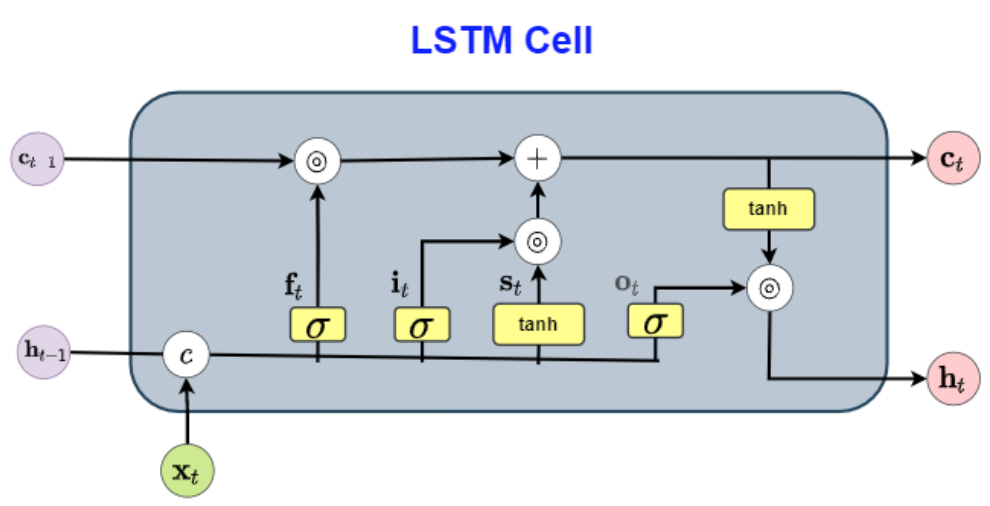
\includegraphics[width=\textwidth]{img/3.3a.png}
     \end{subfigure}
     \hfill
     \begin{subfigure}[b]{0.4\textwidth}
         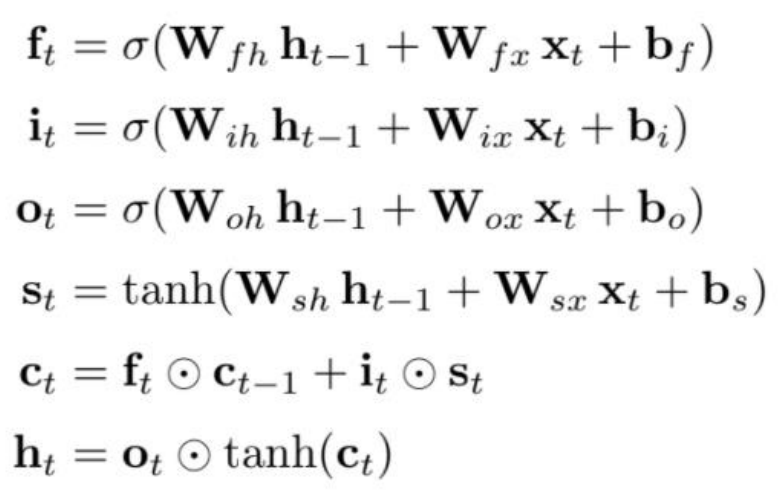
\includegraphics[width=\textwidth]{img/3.3b.png}
     \end{subfigure}
\end{figure}

\mysubsection{1}{What do the gates $f_t, i_t$ and $o_t$ do?}

%\mysubsection{2}{Which of the quantities next to the figure are always positive?}

% Let’s now try to understand how this architecture approaches the vanishing gradients problem. To calculate the gradient $\frac{\partial L}{\partial \theta}$, where $\theta$ stands for the parameters $(W_f, W_o, W_i, W_c)$, we now have to consider the cell state $c_t$ instead of $h_t$. Like $h_t$ in normal RNNs, $c_t$ will also depend on the previous cell states $c_{t-1}, \ldots c_0$, so we get a formula of the form:
% \begin{equation*}
% \frac{\partial L}{\partial W}=\sum^T_{t=0}
% \sum^t_{k=1}
% \frac{\partial L}{\partial c_t}
% \frac{\partial c_t}{\partial c_k}
% \frac{\partial c_k}{\partial W}.
% \end{equation*}

% \mysubsection{2}{We know that $\frac{\partial c_t}{\partial c_k} = \prod^t_{i=k+1} \frac{\partial c_t}{\partial c_{t-1}}$. Let $f_t = 1$ and $i_t = 0$ such that $c_t = c_{t-1}$ for all $t$. What is the gradient $\frac{\partial c_t}{\partial c_k}$ in this case?}

\newpage
\mysubsection{2}{Implement LSTM cell using pytorch tensors. Please create a new cell in the notebook of task 3.5 and write your code there.}

\mysection{3.4. Visualizing Neural Networks\hfill[5]}

In this exercise, you will learn how to visualize the hidden  layers of convolutional neural networks. Follow the instructions in the \texttt{Task3.4\_Visualization.ipynb} notebook and complete all tasks marked as \texttt{TODO}.

\mysection{3.5. NLP with RNNs\hfill[5]}

In this exercise, you will use recurrent neural networks to perform sentiment analysis on Amazon's review dataset. Follow the instructions in the \texttt{Task3.5\_NLP.ipynb} notebook and complete all tasks marked as \texttt{TODO}.

\end{document}